\documentclass[11pt]{article}
\usepackage[pdftex]{graphicx}

\begin{document}
\title{Sieci neuronowe. Projekt}
\author{Micha� Dettlaff}
\maketitle


\section{Wprowadzenie}

\noindent
Celem projektu jest aproksymacja funkcji za pomoc� algorytmu generuj�cego proste regu�y rozmyte
oraz algorytmu propagacji wstecznej.

Aproksymowane s� nast�puj�ce funkcje:

1) $f_1(x) = sin(x) + \epsilon, x \in [0, 2 \pi] $

$ \epsilon $ jest szumem

2) $f_2(x) = exp \left[ -2 log(2) \left(\frac {x - 0.08} {0.854}\right)^2 \right]  sin^6 \left( 5 \pi \left( x^{3/4} - 0.05 \right) \right), x \in [0, 1] $

3) $f_3(x, y) = 200 - (x^2 + y - 11)^2 - (x + y^2 - 7),        x, y \in [-5, 5] $


\section{Metodologia}
\noindent
Metodologia...


\section{Wyniki}

Proste regu�y rozmyte
\begin{center}
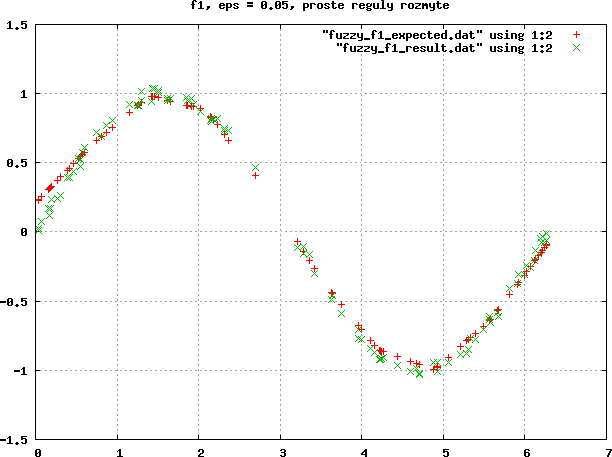
\includegraphics[scale=0.5]{fuzzy_f1}\newline
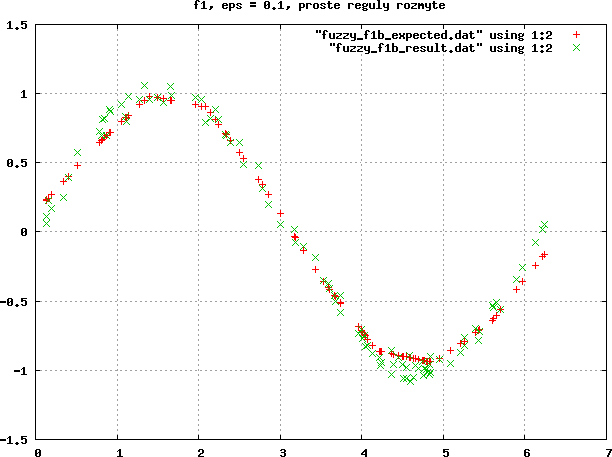
\includegraphics[scale=0.5]{fuzzy_f1b}\newline
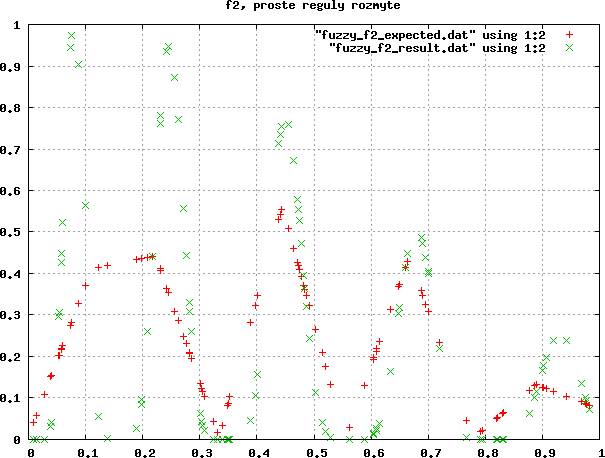
\includegraphics[scale=0.5]{fuzzy_f2}\newline
\end{center}

\newpage
Algorytm propagacji wstecznej
\begin{center}
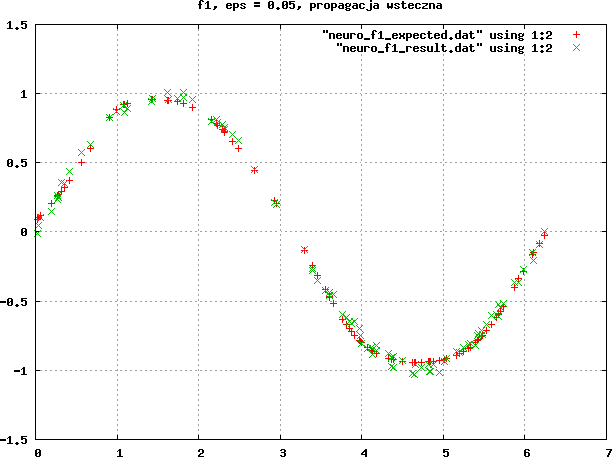
\includegraphics[scale=0.5]{neuro_f1}\newline
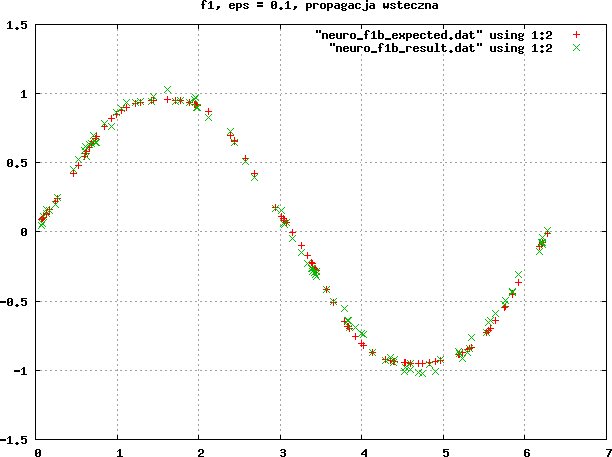
\includegraphics[scale=0.5]{neuro_f1b}\newline
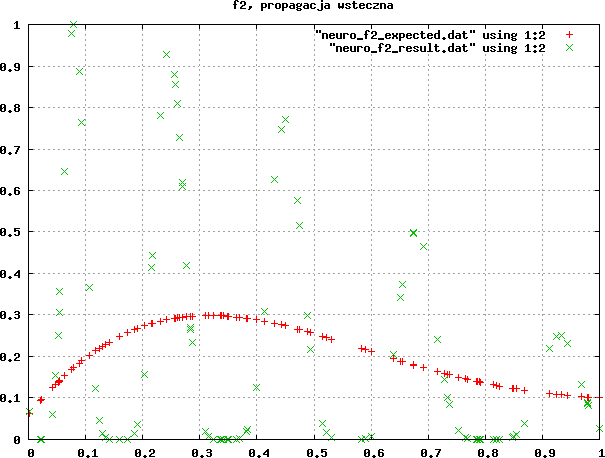
\includegraphics[scale=0.5]{neuro_f2}\newline
\end{center}


\end{document}
